% DO NOT COMPILE THIS FILE DIRECTLY!
% This is included by the other .tex files.

\begin{frame}[t,plain]
\titlepage
\end{frame}

\begin{frame}
    \frametitle{Content of the presentation}
    \huge
    \begin{enumerate}
        \item Automation in MISP
        \vspace{0.5em}
        \item MISP Workflows
        \begin{itemize}
            \Large
            \item Fundamentals
            \item Demo with examples
            \item Using the system
            \item How it can be extended
        \end{itemize}
    \end{enumerate}
\end{frame}

\begin{frame}
    \frametitle{Automation in MISP: What already exists?}
    
\includegraphics[valign=m,width=16px]{pictures/python-logo.png}\hspace*{0.5em} \textbf{MISP API / PyMISP}
    \hspace*{0.25em}
    \begin{itemize}
        \small
        \item Needs CRON Jobs in place
        \item Potentially heavy for the server
        \item Not realtime
    \end{itemize}
    \vspace*{1em}
    
\includegraphics[valign=m,width=16px]{pictures/zeromq.png}\hspace*{0.5em} \textbf{PubSub channels}
    \hspace*{0.25em}
    \begin{itemize}
        \small
        \item After the actions happen: No feedback to MISP
        \item Tougher to put in place \& to share
        \item Full integration amounts to develop a new tool
    \end{itemize}
    \vspace*{1.5em}
    \begin{large}
        $\rightarrow$ No way to \textbf{prevent} behavior\\
        $\rightarrow$ Difficult to setup \textbf{hooks} to execute callbacks
    \end{large}
\end{frame}

\begin{frame}
    \frametitle{Simple automation in MISP made easy}
    \begin{center}
        
\includegraphics[width=0.3\linewidth]{pictures/automation.png}
    \end{center}
    \begin{itemize}
        \item \textbf{Visual} dataflow programming
        \item \textbf{Drag \& Drop} editor
        \item Flexible \textbf{Plug \& Play} system
        \item \textbf{Share} workflows, \textbf{debug} and \textbf{replay}
    \end{itemize}
\end{frame}

\begin{frame}
    \frametitle{Example of use-cases}
    \begin{itemize}
        \item \textbf{Notification} on specifc actions
        \begin{itemize}
            \item New events matching criteria
            \item New users
            \item Automated alerts for high-priority IOCs
        \end{itemize}
        \item \textbf{Extend} existing MISP behavior
        \begin{itemize}
            \item Push data to another system
            \item Automatic enrichment
            \item Sanity check to block publishing / sharing
            \item Curation pipelines
        \end{itemize}
        \item \textbf{Hook} capabilities
        \begin{itemize}
            \item Assign tasks and notify incident response team members
        \end{itemize}
        \item ...
    \end{itemize}
\end{frame}

% \section{Workflow - Fundamentals}
\begin{frame}
    \frametitle{
        \huge
        Workflow - Fundamentals
        \vspace{1em}
    }
    \textbf{Objective:} Start with the foundation to understand the basics
    \begin{center}
        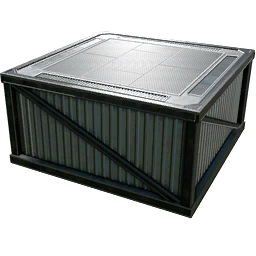
\includegraphics[width=0.07\linewidth]{pictures/fundation}
    \end{center}
\end{frame}


\begin{frame}
    \frametitle{How does it work}
    \begin{center}
        \frame{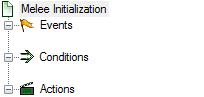
\includegraphics[width=0.6\linewidth]{pictures/event-condition-action.png}}
    \end{center}
    \begin{enumerate}
        \item An \textbf{event} happens in MISP
        \item \textit{\scriptsize (optional)} Check if all \textbf{conditions} are satisfied
        \item Execute all \textbf{actions}
        \begin{itemize}
            \item May prevent MISP to complete its original event
        \end{itemize}
    \end{enumerate}
\end{frame}

\begin{frame}
    \frametitle{What kind of events?}
    
\includegraphics[width=60px]{pictures/sc-event.png}
    \vspace*{0.5em}
    \begin{itemize}
        \item New MISP Event
        \item Attribute has been saved
        \item New discussion post
        \item New user created
        \item Query against third-party services
        \item ...
    \end{itemize}
    \vspace*{1em}
    {\Large \faIcon{question-circle}} Supported events in MISP are called \textbf{Triggers}\\
    {\Large \faIcon{question-circle}} A \textbf{Trigger} is associated with \textbf{1-and-only-1 Workflow}
\end{frame}

\begin{frame}
    \frametitle{Triggers currently available}
    Currently 11 triggers can be hooked. 3 being 
\includegraphics[width=36px]{pictures/blocking-workflow.png}.
    \begin{center}
        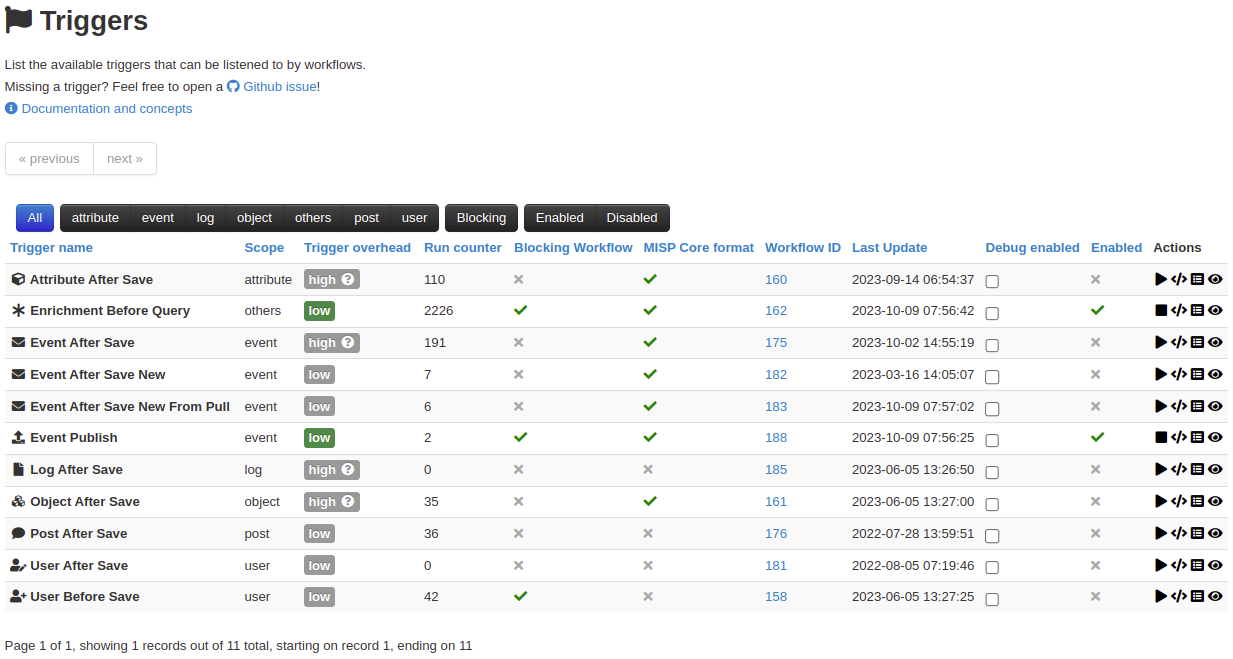
\includegraphics[width=1.0\linewidth]{pictures/triggers.png}
    \end{center}
\end{frame}

\begin{frame}
    \frametitle{What kind of conditions?}
    \vspace*{0.25em}
    
\includegraphics[width=70px]{pictures/sc-condition.png}
    \vspace*{0.25em}
    \begin{itemize}
        % \colorbox{red!100}{\textcolor{white}{\texttt{tlp:red}}}
        \item A MISP Event is tagged with \texttt{tlp:red}
        \item The distribution of an Attribute is a sharing group
        \item The creator organisation is \texttt{circl.lu}
        \item Or any other \textbf{generic} conditions
    \end{itemize}

    \vspace*{0.5em}
    {\Large \faIcon{question-circle}} These are also called \textbf{Logic modules}
    \begin{center}
        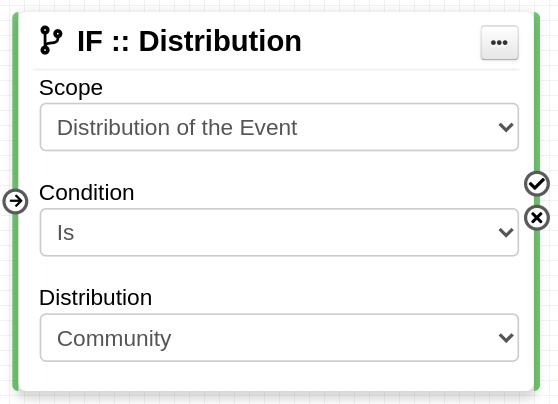
\includegraphics[width=0.43\textwidth]{pictures/logic-module.png}
    \end{center}
\end{frame}

\begin{frame}
    \frametitle{Workflow - Logic modules}
    \begin{itemize}
        \item 
\includegraphics[width=12px]{pictures/sc-condition-icon.png} \textbf{logic} modules: Allow to redirect the execution flow.
        \begin{itemize}
            \item IF conditions
            \item Delay execution
        \end{itemize}
    \end{itemize}
    \begin{center}
        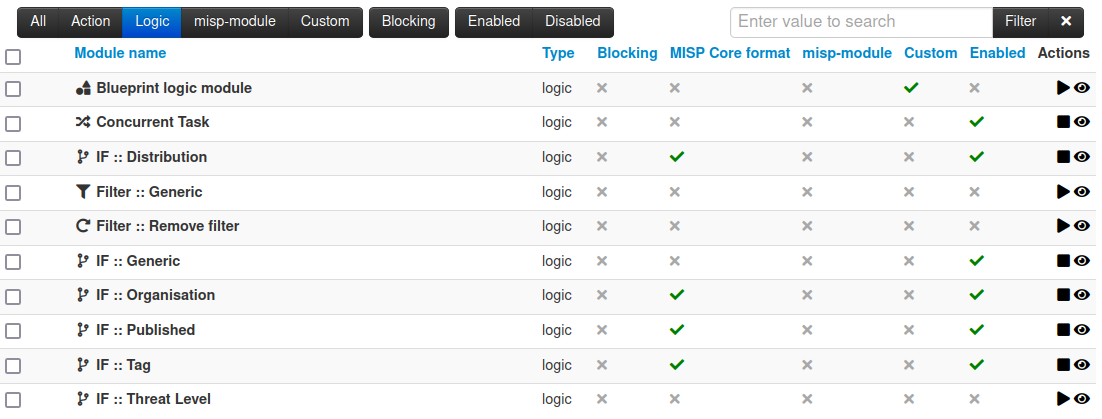
\includegraphics[width=1.0\linewidth]{pictures/logic-module-index.png}
    \end{center}
\end{frame}

\begin{frame}
    \frametitle{What kind of actions?}
    \vspace*{0.25em}
    
\includegraphics[width=60px]{pictures/sc-action.png}
    \vspace*{0.25em}
    \begin{itemize}
        \item Send an email notification
        \item Perform enrichments
        \item Send a chat message on MS Teams
        \item Attach a local tag
        \item ...
    \end{itemize}

    \vspace*{0.5em}
    {\Large \faIcon{question-circle}} These are also called \textbf{Action modules}
    \begin{center}
        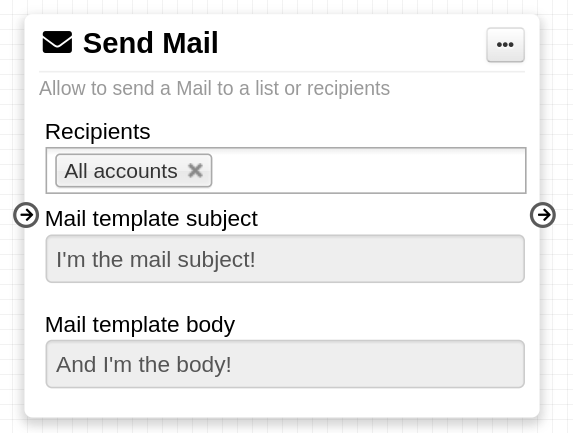
\includegraphics[width=0.43\textwidth]{pictures/action-module.png}
    \end{center}
\end{frame}

\begin{frame}
    \frametitle{Workflow - Action modules}
    \begin{itemize}
        \item 
\includegraphics[width=12px]{pictures/sc-action-icon.png} \textbf{action} modules: Allow to executes operations
        \begin{itemize}
            \item Tag operations
            \item Send notifications
            \item Webhooks \& Custom scripts
        \end{itemize}
    \end{itemize}
    \begin{center}
        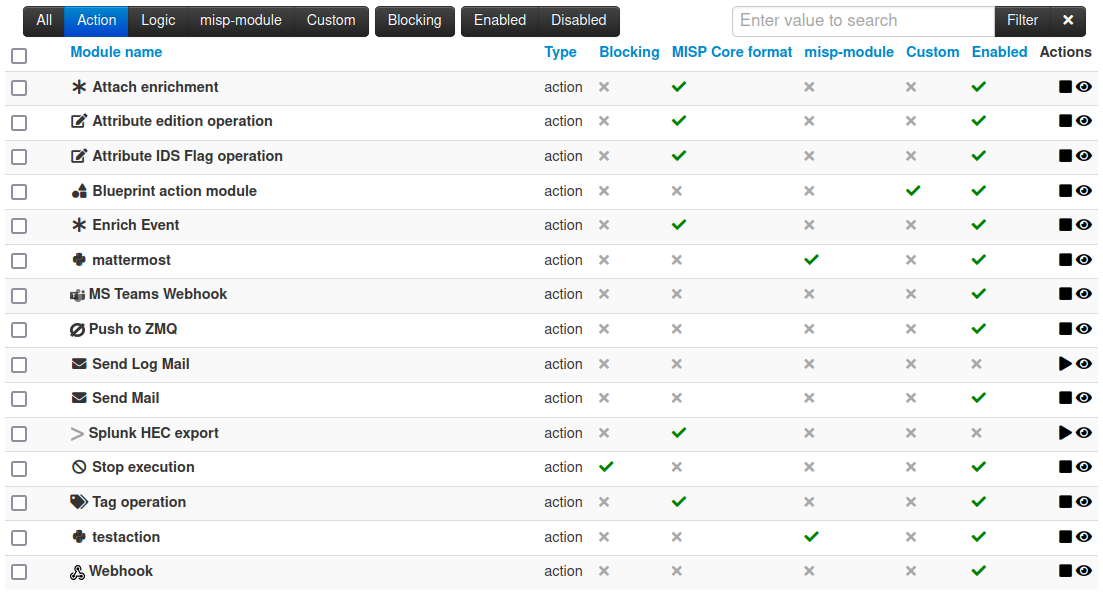
\includegraphics[width=0.95\linewidth]{pictures/action-module-index.png}
    \end{center}
\end{frame}

\begin{frame}
    \frametitle{What is a MISP Workflow?}
    \begin{itemize}
        \item Sequence of all nodes to be executed in a specific order
        \item Workflows can be enabled / disabled
        \item A Workflow is associated to \textbf{1-and-only-1 trigger}
    \end{itemize}
    \vspace*{0.5em}
    \begin{center}
        \frame{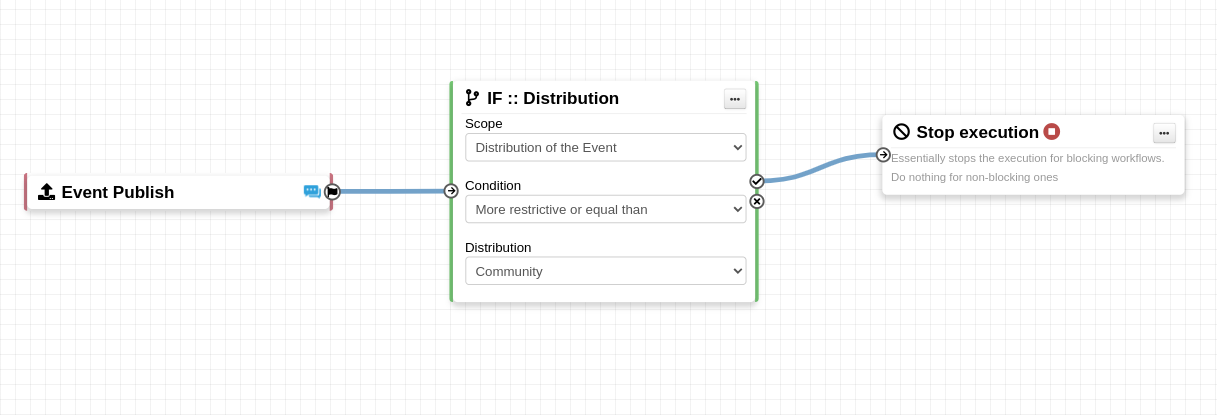
\includegraphics[width=1.0\linewidth]{pictures/simple-workflow.png}}
    \end{center}
\end{frame}

\begin{frame}
    \frametitle{Sources of Workflow modules (0)}
    Currently 36 built-in modules.
    \vspace{1em}
    \begin{itemize}
        \item \textbf{Trigger} module (11): built-in \textbf{only}
        \begin{itemize}
            \item Get in touch if you want more
        \end{itemize}
        \item \textbf{Logic} module (10): built-in \& \textbf{custom}
        \item \textbf{Action} module (20): built-in \& \textbf{custom}
    \end{itemize}
    \vspace*{2.0em}
\end{frame}

\begin{frame}
    \frametitle{Sources of Workflow modules (1)}
    \begin{itemize}
        \item Built-in \textbf{default} modules
        \begin{itemize}
            \item Part of the MISP codebase
            \item Get in touch if you want us to increase the selection (or merge PR!)
        \end{itemize}
    \end{itemize}
    \vspace*{0.5em}
    \begin{center}
        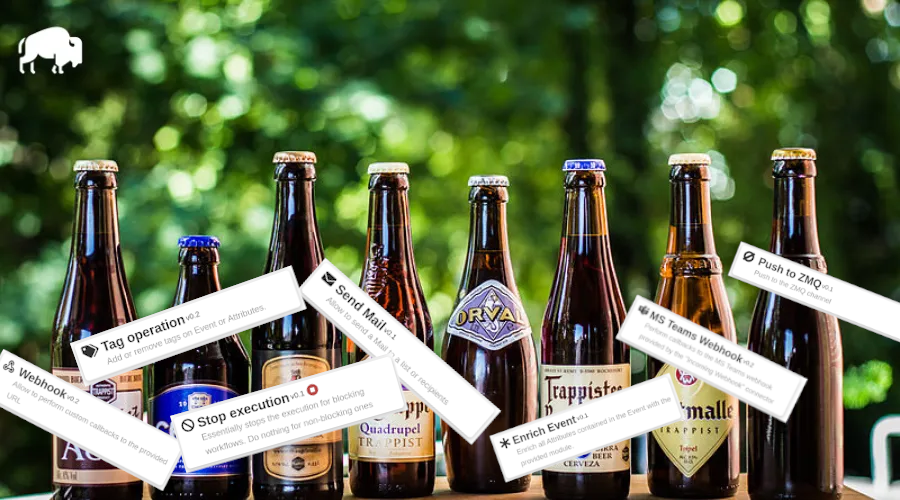
\includegraphics[width=0.8\linewidth]{pictures/module-buffet.png}
    \end{center}
\end{frame}

\begin{frame}
    \frametitle{Sources of Workflow modules (2)}
    User-defined \textbf{custom} modules
    \vspace*{0.5em}
    \begin{columns}
        \begin{column}{0.5\textwidth}
            \begin{itemize}
                \item Written in PHP
                \item Extend existing modules
                \item MISP code reuse
            \end{itemize}
        \end{column}
        \begin{column}{0.5\textwidth}
            
\includegraphics[width=1.0\linewidth]{pictures/php-joke.jpg}
        \end{column}
    \end{columns}
\end{frame}

\begin{frame}
    \frametitle{Sources of Workflow modules (3)}
    Modules from the 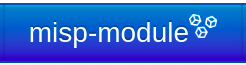
\includegraphics[width=0.20\linewidth]{pictures/misp-module-icon.png} \textbf{enrichment service}
    \vspace*{0.5em}
    \begin{columns}
        \begin{column}{0.50\textwidth}
            \begin{itemize}
                \item Written in Python
                \item Can use any python libraries
                \item Plug \& Play
            \end{itemize}
        \end{column}
        \begin{column}{0.50\textwidth}
            
\includegraphics[width=1.0\linewidth]{pictures/python-joke.png}
        \end{column}
    \end{columns}
\end{frame}

\begin{frame}
    \frametitle{Demo by examples}
    \begin{enumerate}
        \item[WF-1.] Send an email to \textbf{all admins} when a new event has been pulled
        \vspace*{2em}
        \item[WF-2.] Block queries on 3rd party services when \textbf{tlp:red} or \textbf{PAP:red}
        \begin{itemize}
            \item \textbf{tlp:red}: For the eyes and ears of individual recipients only
            \item \textbf{PAP:RED}: Only passive actions that are not detectable from the outside
        \end{itemize}
    \end{enumerate}
\end{frame}

\begin{frame}
    \frametitle{Demo WF-1: Send an email to \textbf{all admins} when a new event has been pulled}
     \begin{center}
        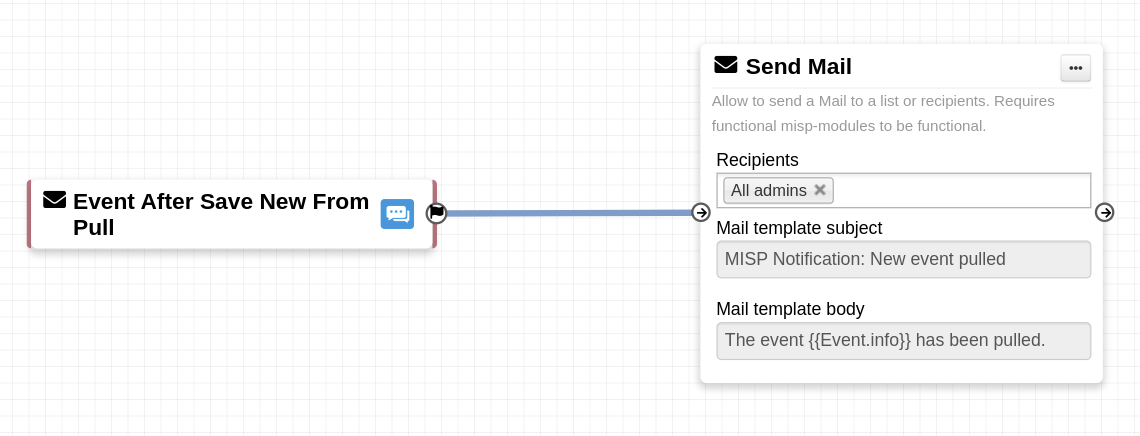
\includegraphics[width=1.0\linewidth]{pictures/demo-wf1.png}
    \end{center}
\end{frame}

\begin{frame}
    \frametitle{Demo WF-2: Block queries on 3rd party services when \textbf{tlp:red} or \textbf{PAP:red}}
    \begin{itemize}
        \small
        \item \textbf{tlp:red}: For the eyes and ears of individual recipients only
        \item \textbf{PAP:RED}: Only passive actions that are not detectable from the outside
    \end{itemize}
    \vspace*{1em}
     \begin{center}
        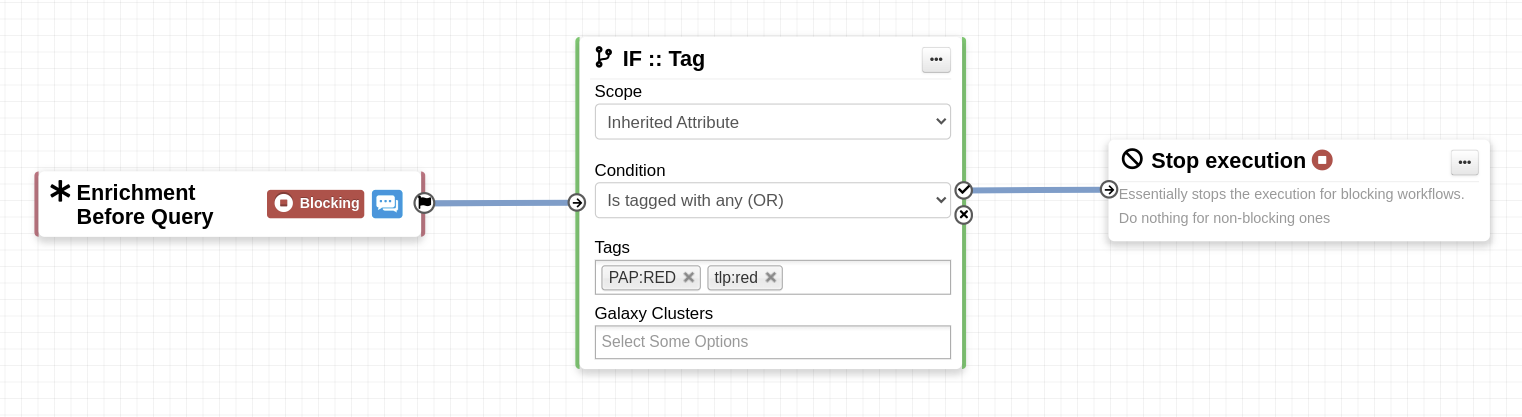
\includegraphics[width=1.0\linewidth]{pictures/demo-wf2.png}
    \end{center}
\end{frame}

\begin{frame}
    \frametitle{Getting started with workflows}
    \centering
    {\Large Everything is ready?}\\
    \vspace*{3em}
    {\LARGE Let's see how to build a workflow!}
    \begin{center}
        
\includegraphics[width=24px]{pictures/build-icon.png}
    \end{center}
\end{frame}

\begin{frame}
    \frametitle{Creating a workflow with the editor}
    \begin{enumerate}
        \item \underline{Prevent} event publication \texttt{\bf \large if tlp:red} tag
        \begin{itemize}
            \item \underline{Send a mail} to \texttt{\scriptsize admin@admin.test} about potential data leak
        \end{itemize}
        \item \texttt{\bf \large else}, \underline{send a notification} on Mattermost
    \end{enumerate}
\end{frame}

% \section{Considerations when working with workflows}
\begin{frame}
    \frametitle{
        \huge
        Considerations when working with workflows
        \vspace{1em}
    }
    \textbf{Objective:} Overview of some common pitfalls
    \begin{center}
        
\includegraphics[width=24px]{pictures/radar.png}
    \end{center}
\end{frame}

\begin{frame}
    \frametitle{Working with the editor - Operations not allowed}
    Execution loop are not authorized
    \vspace*{1em}
    \begin{columns}
        \begin{column}{0.7\textwidth}
            \frame{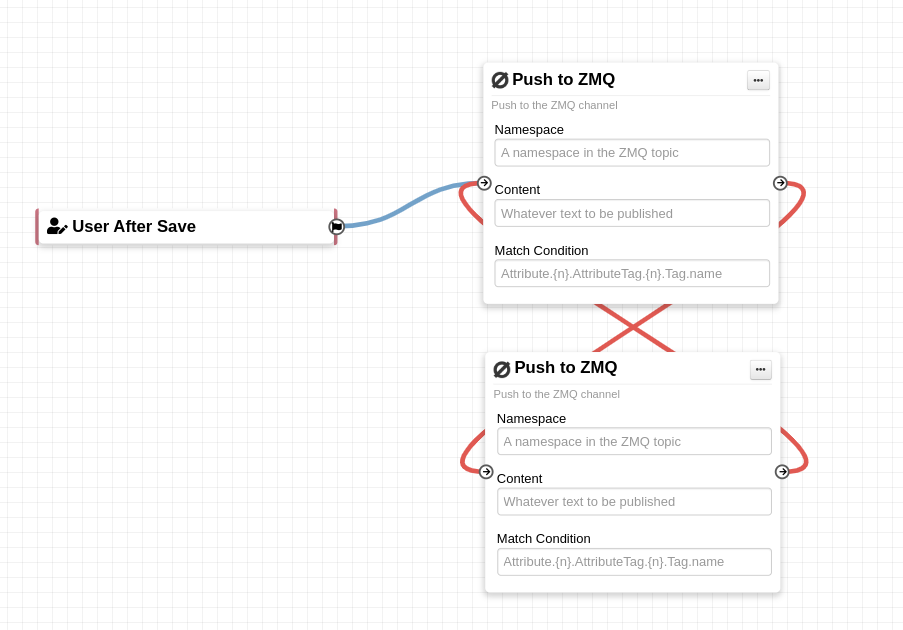
\includegraphics[width=1.0\linewidth]{pictures/editor-not-allowed-1.png}}
        \end{column}
        \begin{column}{0.3\textwidth}
            \frame{
\includegraphics[width=1.0\linewidth]{pictures/infinite-loop.jpg}}
        \end{column}
    \end{columns}
\end{frame}

\begin{frame}
    \frametitle{Recursive workflows}
    \frame{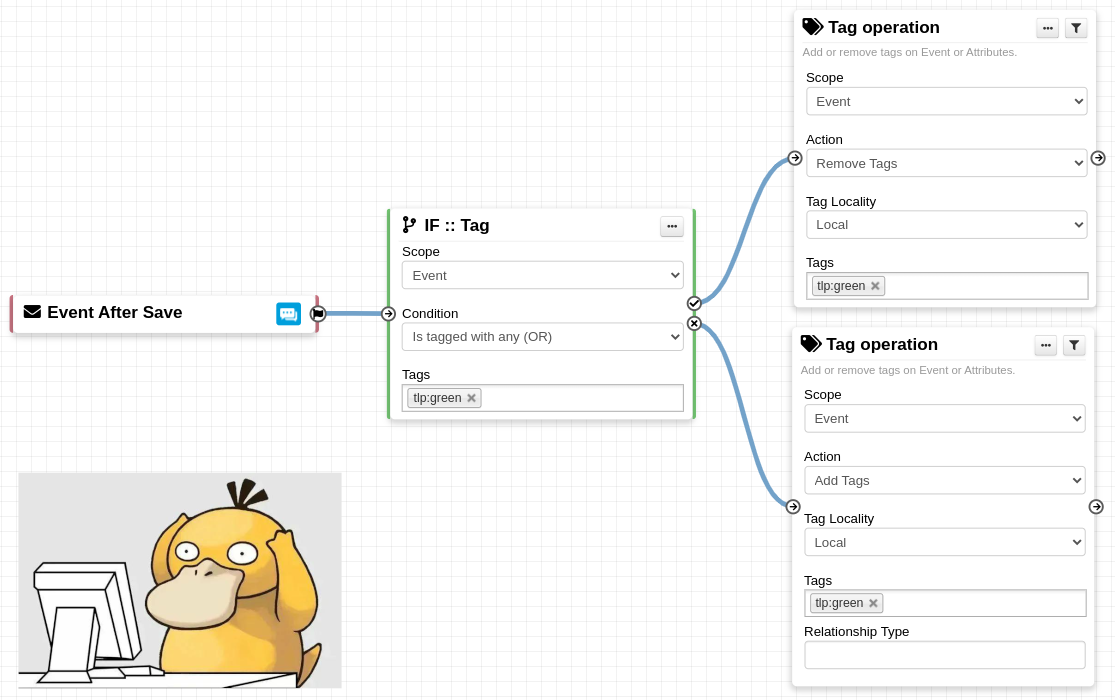
\includegraphics[width=1.0\linewidth]{pictures/recursive-workflow.png}}
    \danger Recursion: If an action re-run the workflow
\end{frame}

\begin{frame}
    \frametitle{Working with the editor - Operations not allowed}
    Multiple connections from the same output
    \vspace*{1em}
    \begin{columns}
        \begin{column}{0.7\textwidth}
            \frame{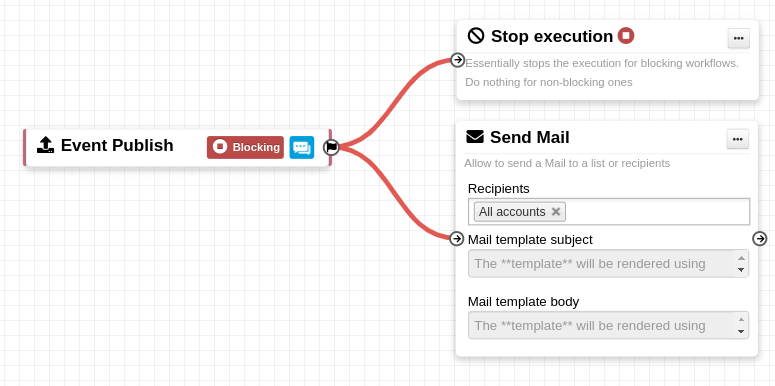
\includegraphics[width=1.0\linewidth]{pictures/editor-not-allowed-2.png}}
        \end{column}
        \begin{column}{0.3\textwidth}
            \frame{
\includegraphics[width=1.0\linewidth]{pictures/two-paths.jpeg}}
        \end{column}
    \end{columns}
    \begin{itemize}
        \item Execution order not guaranted
        \item Confusing for users
    \end{itemize}
\end{frame}


% \section{Advanced usage}
\begin{frame}
    \frametitle{
        \huge
        Advanced usage
        \vspace{1em}
    }
    \textbf{Objective:} Overview of Blueprints, Data format and Filtering
\end{frame}

\begin{frame}
    \frametitle{Workflow blueprints}
    \begin{enumerate}
        \item Blueprints allow to \textbf{re-use parts} of a workflow in another one
        \item Blueprints can be saved, exported and \textbf{shared}
    \end{enumerate}
    \begin{center}
        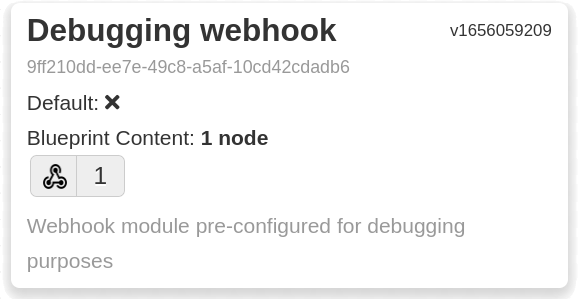
\includegraphics[width=0.5\linewidth]{pictures/blueprint-debugging.png}
    \end{center}
    Blueprints sources: \texttt{\scriptsize MISP/misp-workflow-blueprints} repository\footnote{\scriptsize https://github.com/MISP/misp-workflow-blueprints}
    \begin{itemize}
        \small
        \item Block actions if any attributes have the \texttt{PAP:RED} or \texttt{tlp:red} tag
        \item Curation pipeline
        \item Enrich data from 3rd-party
    \end{itemize}
\end{frame}

\begin{frame}
    \frametitle{Fitlering data on which to apply a module}
    What is the outcome of executing this workflow?
    \begin{center}
        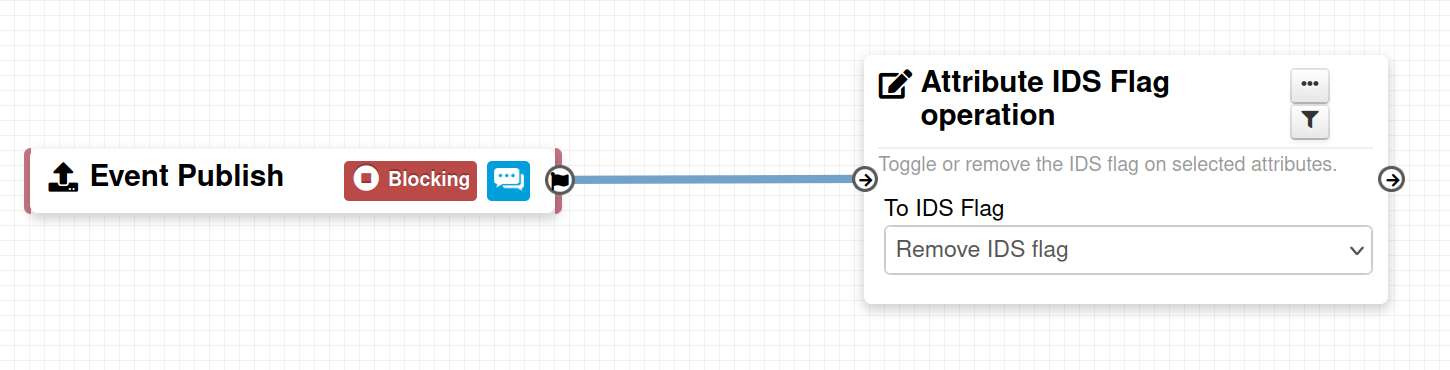
\includegraphics[width=1.0\textwidth]{pictures/remove-ids-1.png}
    \end{center}
    \pause
    \vspace{1em}
    All Attributes get their \texttt{to\_ids} turned off.\\
    \vspace{1em}
    How could we force that action only on Attribute of type \texttt{comment}?
    \begin{center}
        $\rightarrow$ Hash path filtering!
    \end{center}
\end{frame}

\begin{frame}
    \frametitle{Fitlering data on which to apply a module}
    \begin{center}
        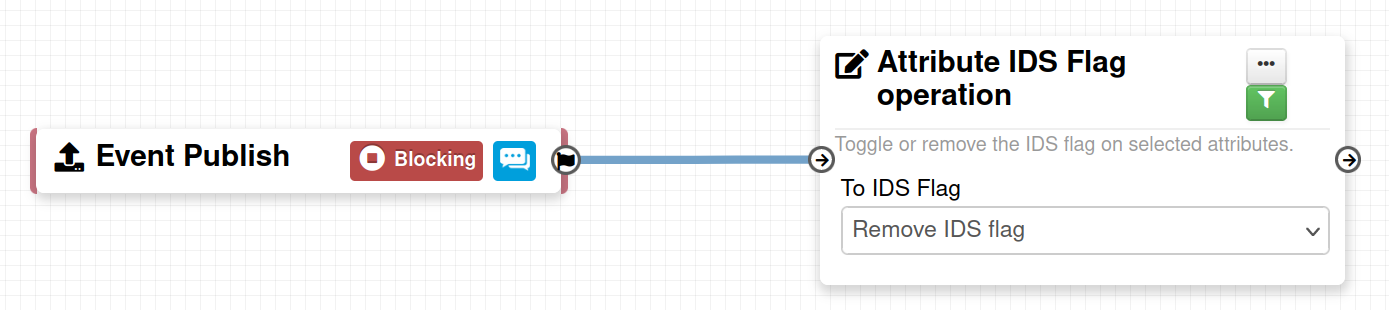
\includegraphics[width=0.5\textwidth]{pictures/remove-ids-3.png}
    \end{center}
    \begin{center}
        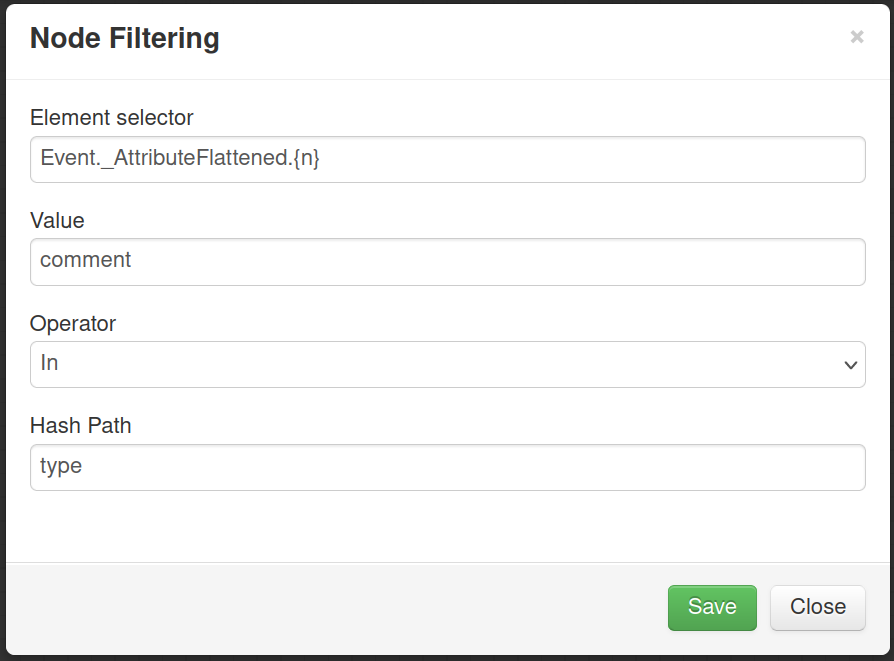
\includegraphics[width=0.9\textwidth]{pictures/remove-ids-2.png}
    \end{center}
\end{frame}

\begin{frame}
    \frametitle{Fitlering data on which to apply a module}
    \begin{center}
        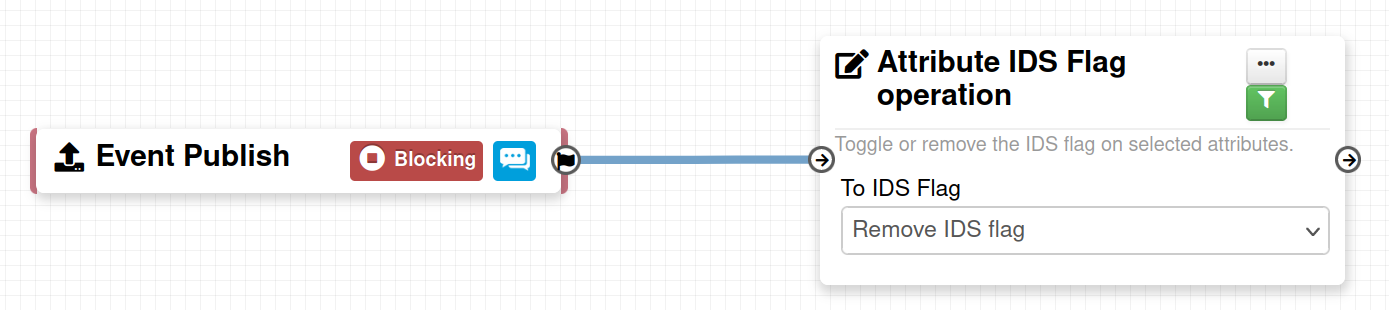
\includegraphics[width=0.5\textwidth]{pictures/remove-ids-3.png}
    \end{center}
    \begin{center}
        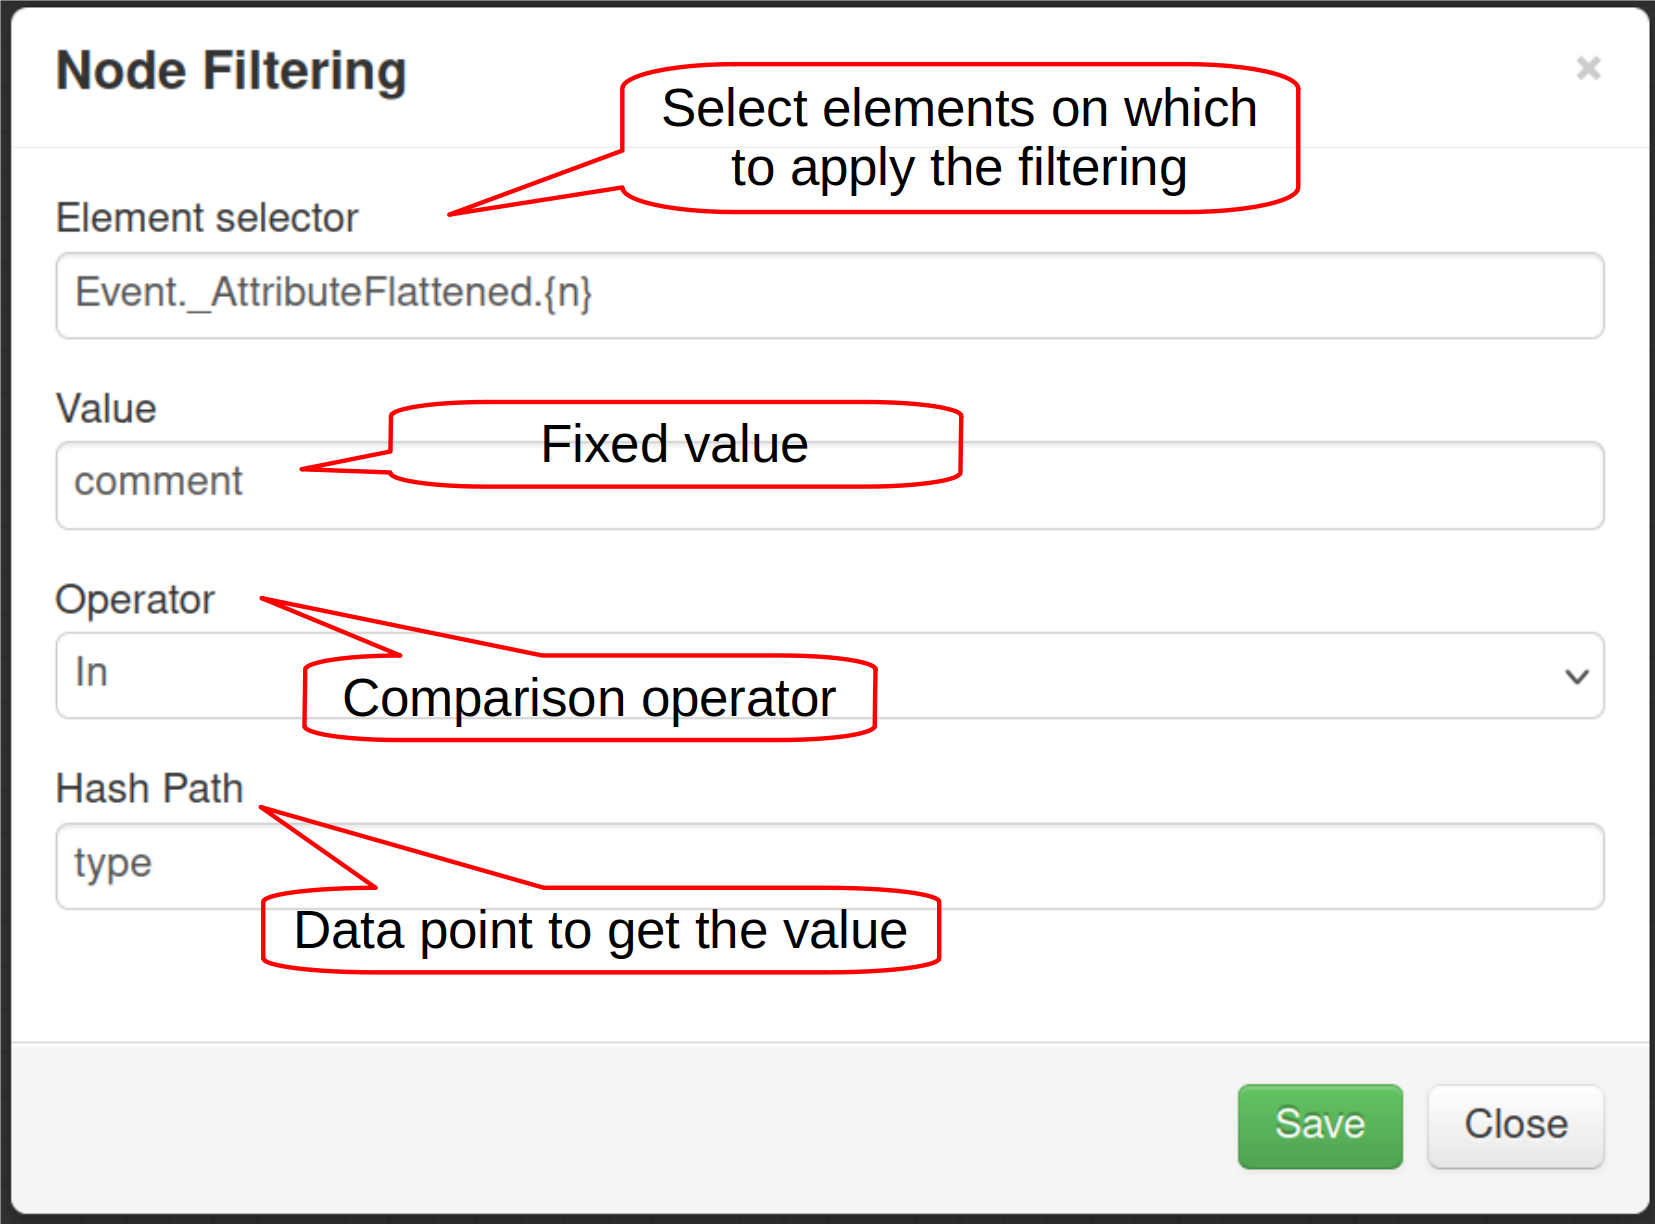
\includegraphics[width=0.9\textwidth]{pictures/remove-ids-2-details.png}
    \end{center}
\end{frame}

\begin{frame}
    \frametitle{Fitlering data on which to apply on multiple modules}
    New feature as of \textbf{v2.4.171} allows setting filters on a path.
    \begin{center}
        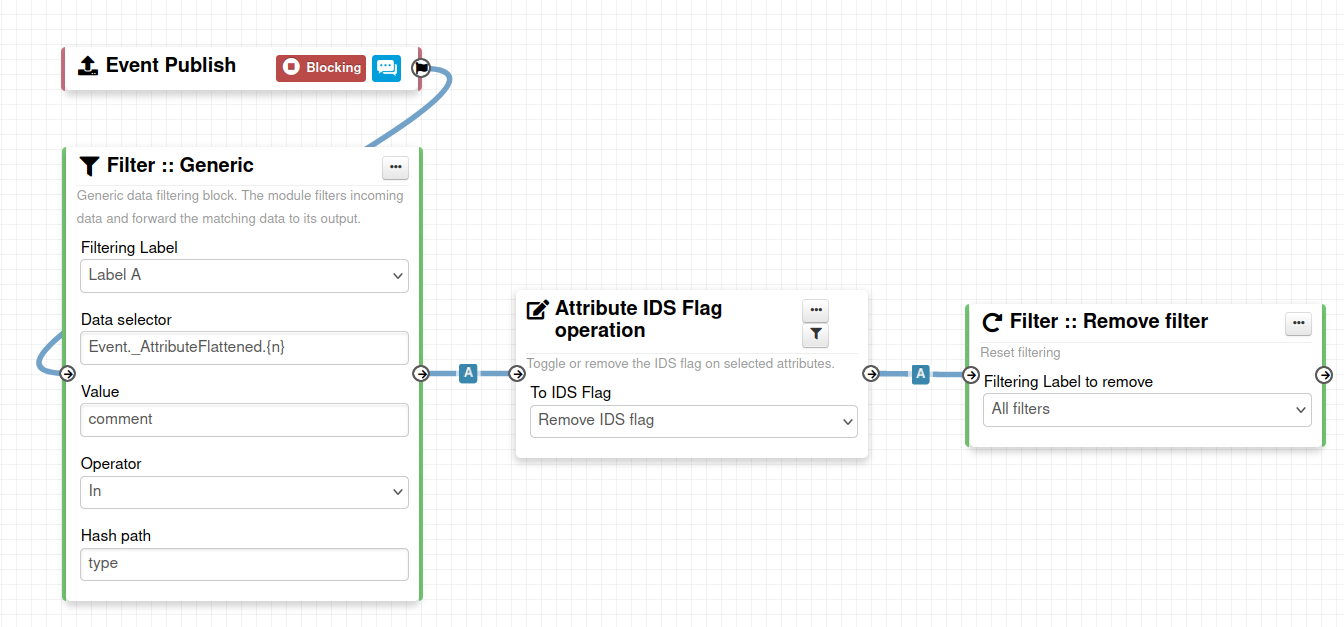
\includegraphics[width=1.0\textwidth]{pictures/remove-ids-generic.png}
    \end{center}
\end{frame}

\begin{frame}
    \frametitle{Should I migrate to MISP Workflows}
    I have automation in place using the API/ZMQ. Should I move to Workflows?
    \vspace{1em}
    \begin{itemize}
        \item I have a curation pipeline using the API, should I port it to workflows?
        \begin{itemize}
            \item \textbf{No} in general, but WF can be used to start the curation process or perform simple pre-processing
        \end{itemize}
        \item What if I want to \textbf{block} some actions
        \begin{itemize}
            \item Put the blocking logic in the WF, keep the remaining outside
        \end{itemize}
        \item Bottom line is \textbf{Keep it simple} for you to maintain
    \end{itemize}
\end{frame}

\begin{frame}
    \frametitle{Future works}
    \begin{columns}
        \begin{column}{0.55\textwidth}
            \begin{itemize}
                \item More 
\includegraphics[width=12px]{pictures/sc-action-icon.png} modules
                \item More 
\includegraphics[width=12px]{pictures/sc-condition-icon.png} modules
                \item More 
\includegraphics[width=12px]{pictures/sc-event-icon.png} triggers
                \item Recursion prevention system
            \end{itemize}
        \end{column}
        \begin{column}{0.45\textwidth}
            
\includegraphics[width=1.0\linewidth]{pictures/future-works.jpeg}
        \end{column}
    \end{columns}
\end{frame}

\begin{frame}
    \frametitle{Final words}
    \begin{columns}
        \begin{column}{0.6\textwidth}
            \begin{itemize}
                \item Designed to \textbf{quickly} and \textbf{cheaply} integrate MISP in CTI pipelines
                \item \underline{\textbf{Beta}} Feature unlikely to change. But still..
                \item Waiting for feedback!
                \begin{itemize}
                    \item New triggers?
                    \item New modules?
                \end{itemize}
            \end{itemize}
        \end{column}
        \begin{column}{0.4\textwidth}
            
\includegraphics[width=1.0\linewidth]{pictures/feeling-of-power.jpg}
        \end{column}
    \end{columns}
    \vspace*{0.5em}
\end{frame}

